%%
%% Author: dariochinelli
%% 2021-04-21
%%

\section{Potenziale nucleare}
Studiamo il potenziale nucleare considerando il nucleo del \emph{deuterio}, chiamato \emph{deutone}, composto da un protone ed un neutrone.

\paragraph{La Cromodinamica Quantistica (QCD)} è una teoria quantistica di campo e relativistica, è una teoria fondamentale che spiega l'interazione tra particelle elementari.
I nucleoni, i componenti del nucleo, protone e neutrone, sono a loro volta composti da \emph{quark}, i quali sono particelle elementari prive di dimensione e con carica frazionaria
\begin{itemize}
\item quark up $u$ ha carica $+\frac{2}{3}$
\item quark down $d$ ha carica $-\frac{1}{3}$
\end{itemize}
i nucleoni sono composti da 3 quark ciascuno e seguono la regola per cui
\begin{itemize}
\item il \textbf{protone} è composto da due quark \emph{up} ed un quark \emph{down}, ha quindi carica totale unitaria:
$$u+u+d = +\frac{2}{3} +\frac{2}{3} -\frac{1}{3} = 1$$
\item il \textbf{neutrone} è composto da due quark \emph{down} ed un quark \emph{up}, ha quindi carica totale nulla:
$$d+d+u = -\frac{1}{3} -\frac{1}{3} +\frac{2}{3} = 0$$
\end{itemize}
\begin{figure}[h]
\centering
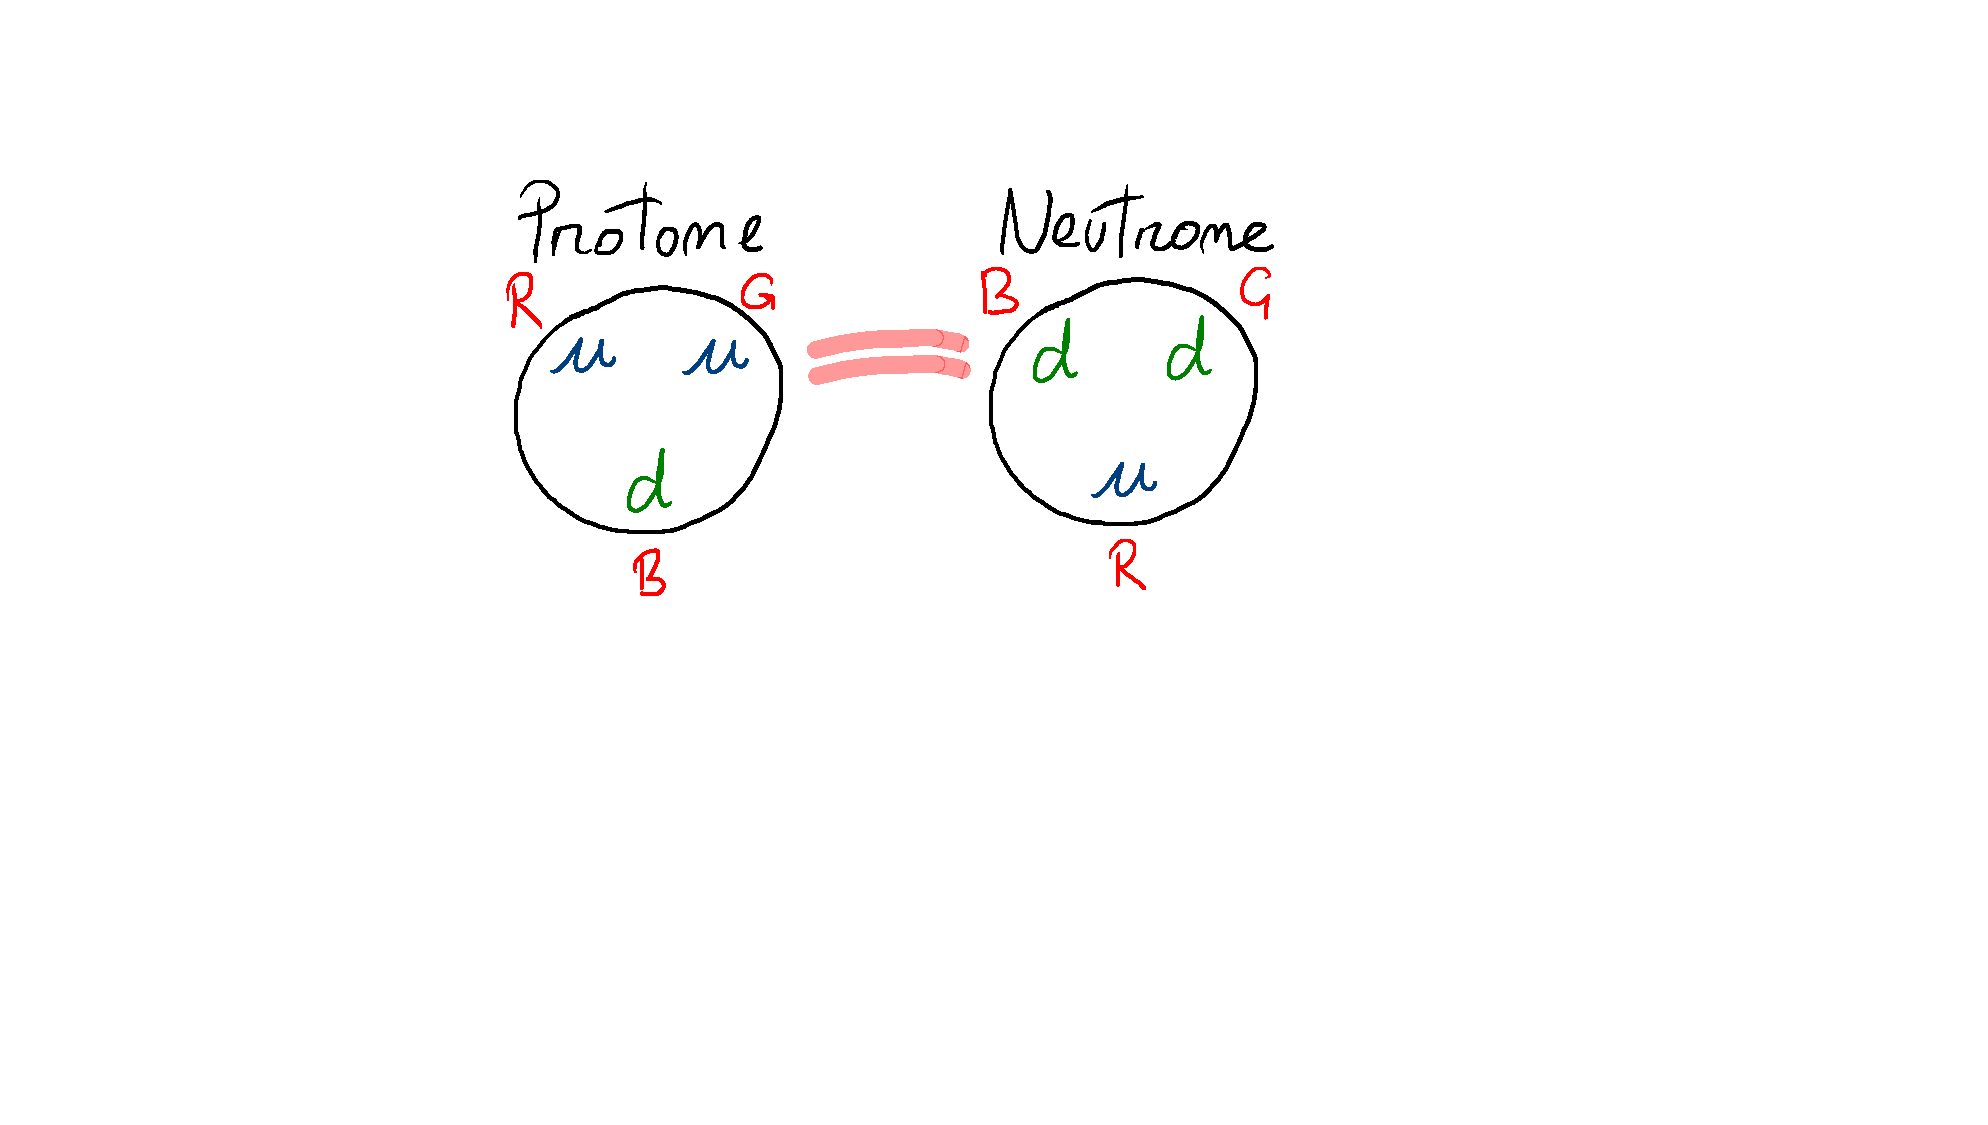
\includegraphics[scale=0.5]{/protone_neutrone_quark}
\caption{CAPTION}
\end{figure}

\paragraph{Carica di colore} I quark hanno anche un secondo tipo di carica: la \emph{carica di colore} che regola l'\emph{interazione forte} tra i quark.
La carica di colore può essere di tre tipi: Red (R), Green (G), Blue (B).
La somma delle tre cariche di colore dei rispettivi quark di un nucleone è nulla
\begin{equation}
R + G + B = 0
\end{equation}
un quark rosso (R) attira un quark verde (G) che attira un quark blu (B), mentre i quark dello stesso colore si respingono.
La teoria fondamentale della QCD esprime come l'interazione nucleare si possa interpretare come la carica di colore residua.

\paragraph{Il potenziale tra nucleoni} è un potenziale di interazione del tipo
\begin{figure}[h]
\centering
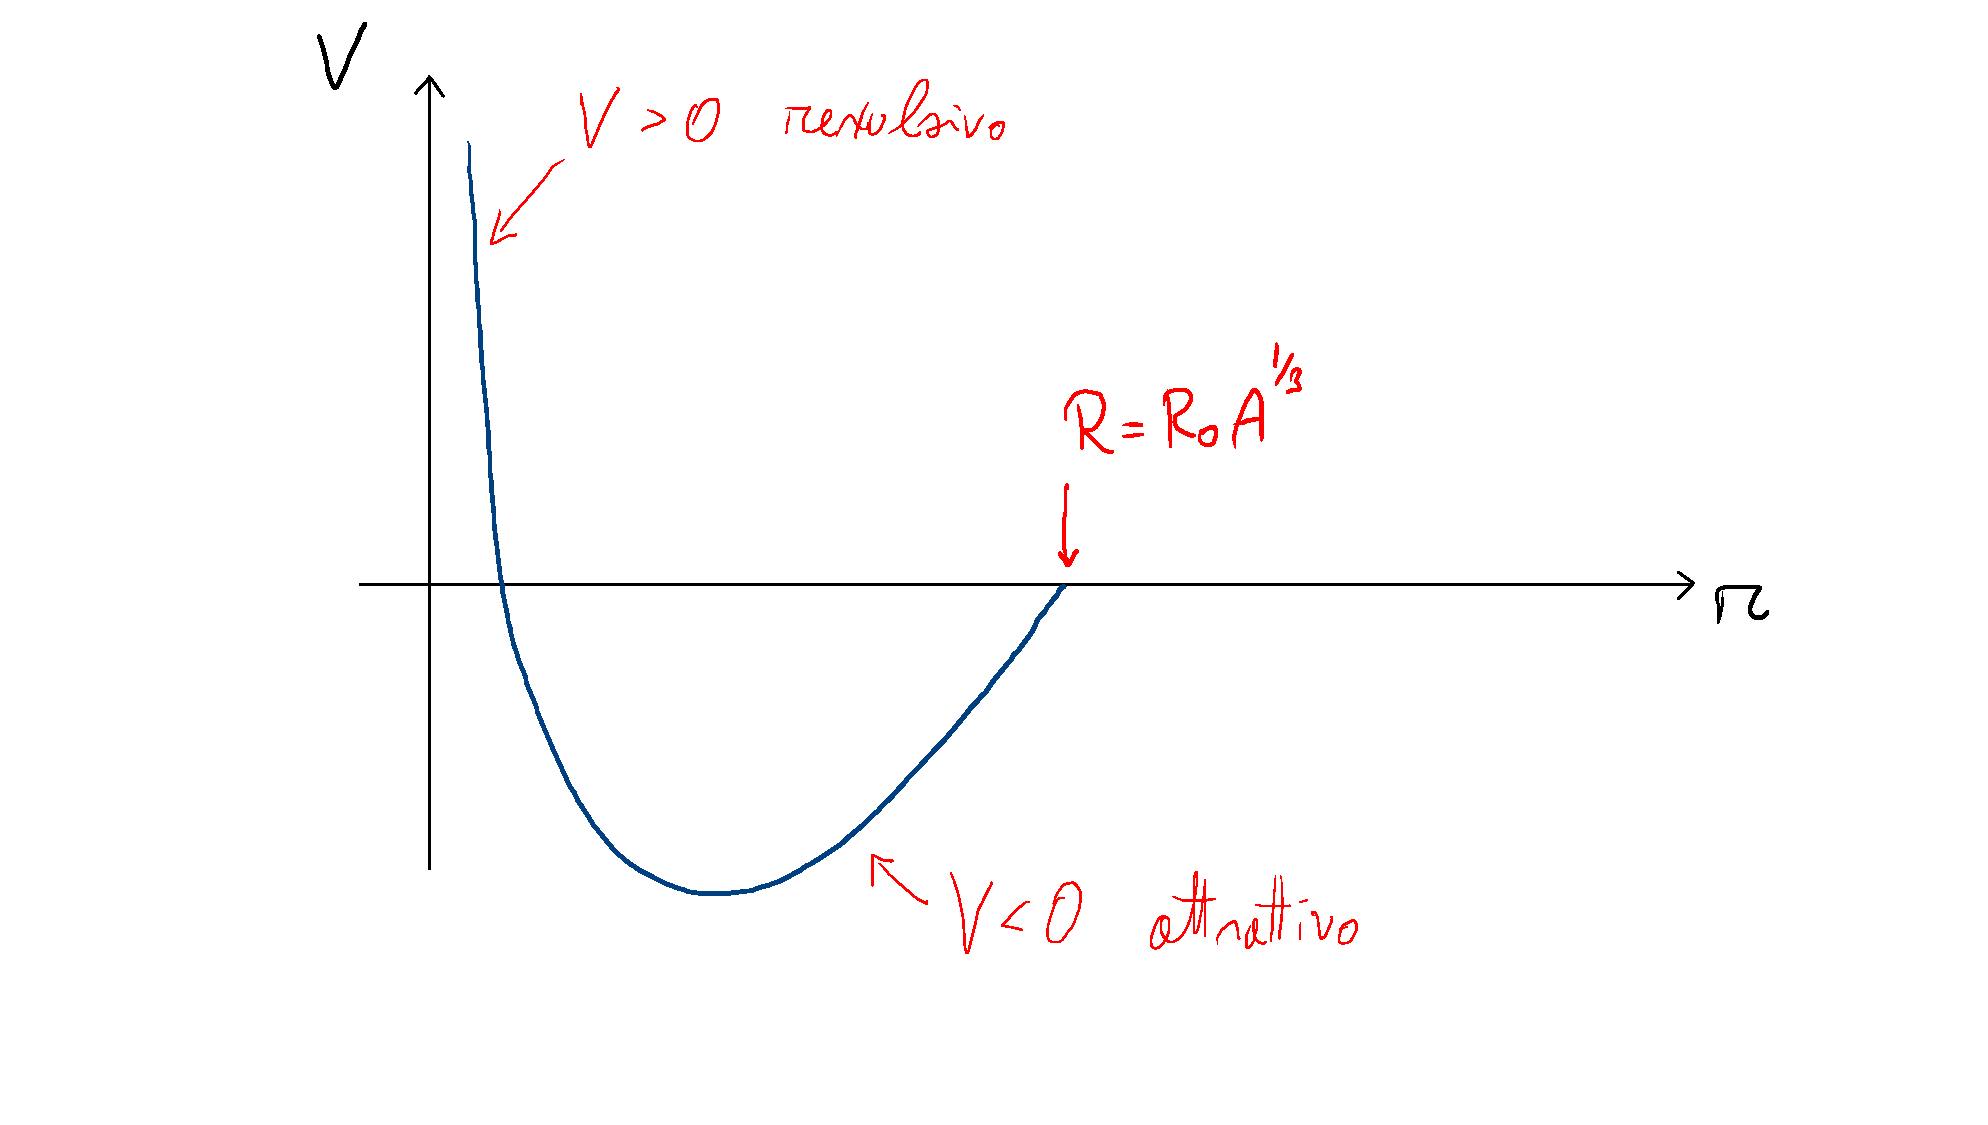
\includegraphics[scale=0.4]{/potenziale_nucleare_1}
\caption{CAPTION}
\end{figure}
Nella prima parte del potenziale si ha che per piccole distanze è \emph{positivo}, ovvero repulsivo, poiché altrimenti i nuclei \underline{privi di dimensione (?)} collasserebbero, ciò è legato al Principio di Esclusione di Pauli, nella seconda parte il potenziale è \emph{attrattivo} ed è ciò che "intrappola" i nucleoni all'interno del nucleo, inoltre oltre alla distanza data da $R = R_0 A^{\frac{1}{3}}$ la forza nucleare è nulla.

\paragraph{Il Deutone} è il nucleo del deuterio, è composto da un protone e un neutrone ed è il più semplice nucleo su cui studiare la forza nucleare.
Del deutone conosciamo l'energia di legame $E_B = \SI{-2.225}{MeV}$ e la distanza tra i nucleoni $R = \SI{2.1}{fm}$ ottenuti sperimentalmente.
Conosciamo inoltre che lo stato legato del deuterio è quello in cui gli spin sono paralleli, dato ottenuto dalla misurazione del momento magnetico, per cui lo spin del deutone è $S = 1$.
\begin{figure}[h]
\centering
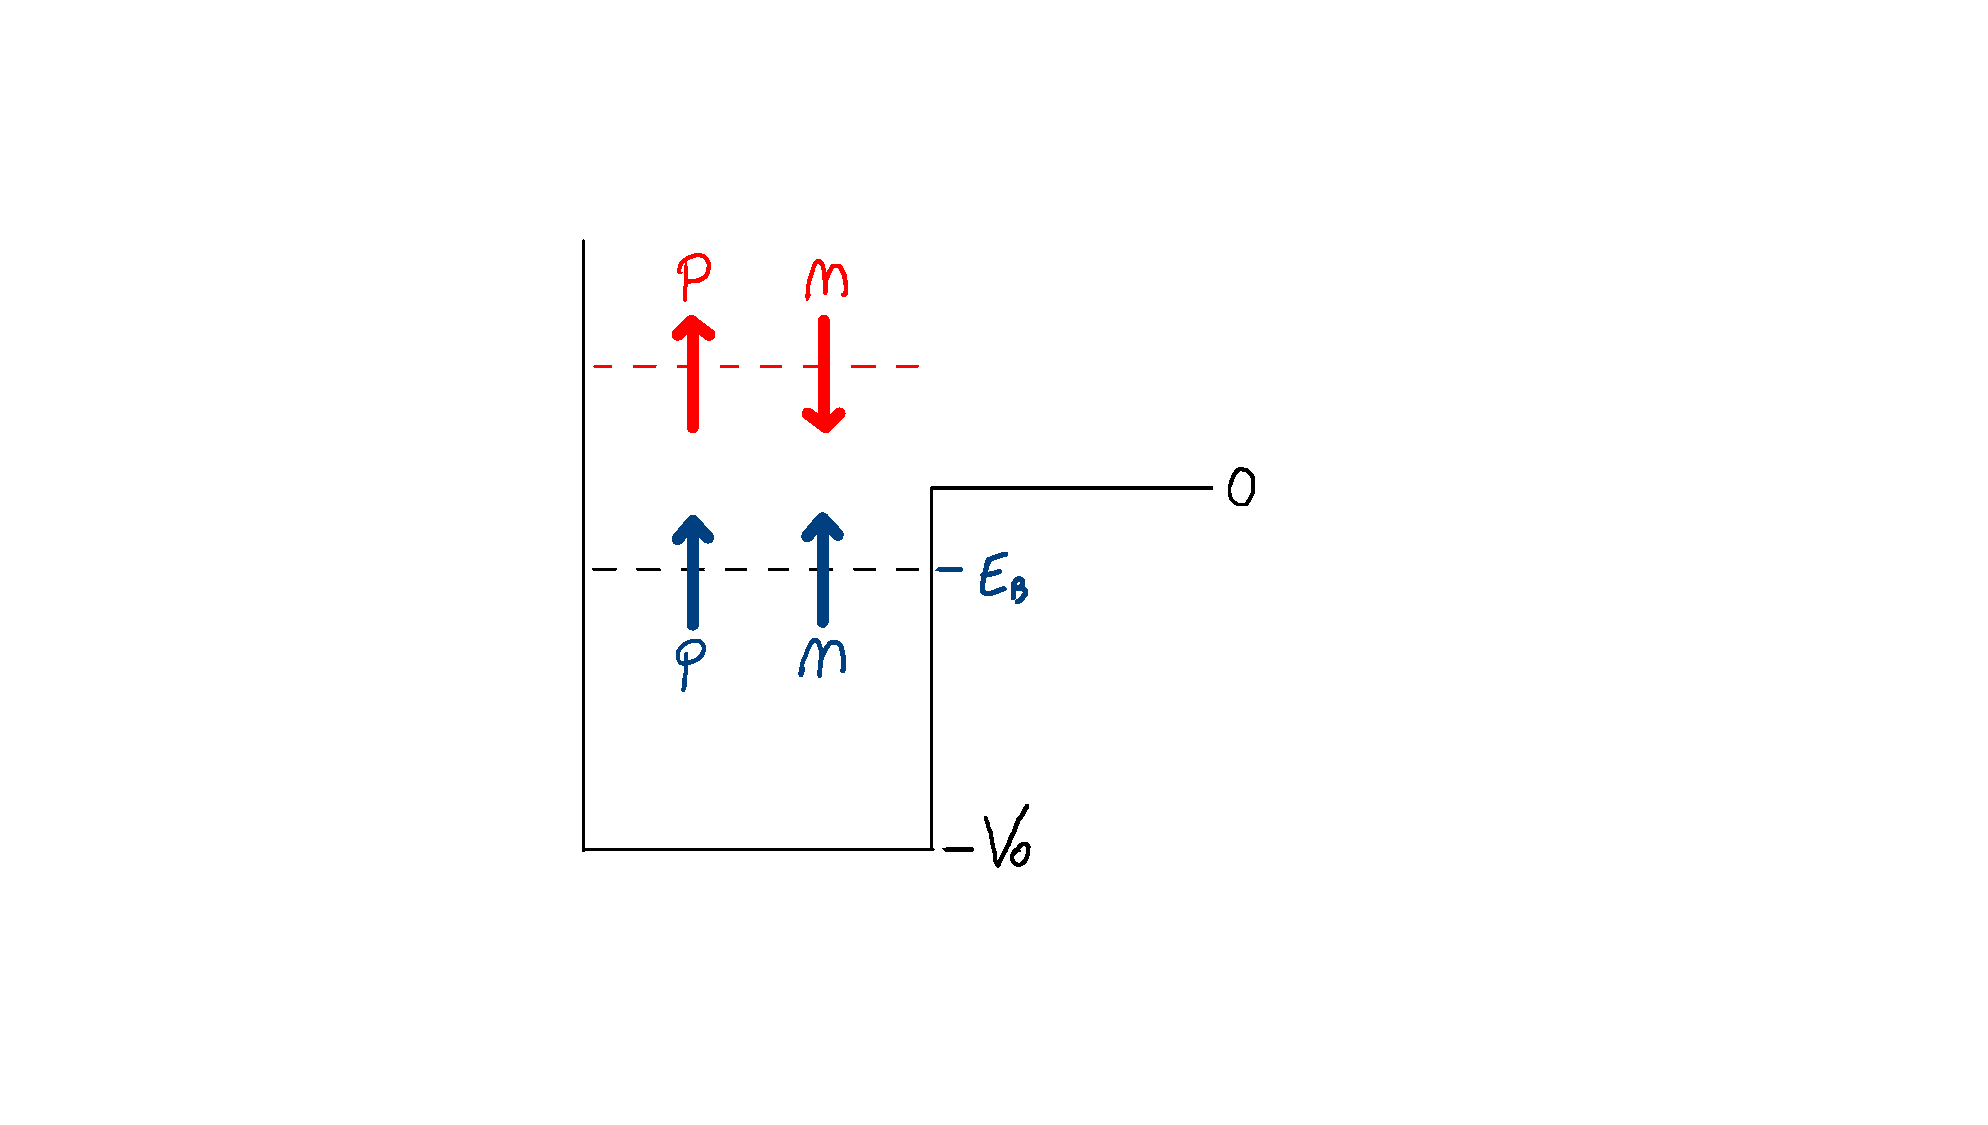
\includegraphics[scale=0.5]{/spin_deutone}
\caption{CAPTION}
\end{figure}
Uno stato con spin anti-parallelo corrisponde ad uno stato non legato, quindi fuori dalla buca di potenziale.
L'interazione nucleare dipende fortemente dallo spin.

Cerco ora il valore della buca di potenziale $V_0$, sommo l'energia cinetica $KE$ con l'energia potenziale $PE$
\begin{equation}
\begin{split}
E & = KE + PE \\
E_B & = KE + V_0
\end{split}
\end{equation}
scrivendo la funzione d'onda trovo il legame con il potenziale $V$
\begin{equation}
\begin{split}
H \psi & = E \psi \\
- \frac{\hbar^2}{2m} \frac{d^2}{dr^2} \psi + V \psi & = E \psi
\end{split}
\end{equation}
Il potenziale in questo esempio si scrive come
\begin{equation}
V = 
\Bigg\{\begin{array}{l}
V_0 \quad\mbox{dentro la buca : zona \Romannum{1}} \\
0 \quad\quad\mbox{altrove : zona \Romannum{2}}
\end{array}
\end{equation}













